% !TeX spellcheck = en_GB
%!TEX root = ../side-constrained.tex

\section{A Counter Example}\label{sec:counter}

We now want to describe the dynamic flow model with hard edge capacities introduced by Zhong, Sumalee, Friesz and Lam~\cite{zhong11}. In order to formally define such edge capacities one first needs to be able to translate the individual particles' strategy choices (i.e. a walk inflow $h$) into the resulting dynamic flow on the edges of the network. This translation process is usually called \emph{network loading} and it typically uses some given edge delay functions $D_e(h,.): \IR_{\geq 0} \to \IR_{\geq 0}$ in order to model the flow dynamics on individual edges. Here, $D_e(h,t)$ denotes the travel time along edge $e$ when entering at time $t$ under the flow induced by $h$.

Using such edge delays, one can define the edge flow corresponding to a given walk inflow $h$: For this we define the set $\mathcal{R} \coloneqq \Set{(p,j) | p \in \Pc, j \in [\abs{p}]}$, i.e. $\mathcal{R}$ contains exactly one element for every walk in $\Pc$ and each of its edges (counted with multiplicity if an edge occurs multiple times on the walk). An edge flow corresponding to a given walk inflow $h$ is then a tuple $(f^+,f^-)$ with $f^+,f^- \in L_+(\IR_{\geq 0})^\mathcal{R}$ satisfying the following conditions:
\begin{itemize}
	\item Correspondence to $h$: 
	\[f^+_{p,1}(\theta) = h_p(\theta) \text{ for all } p \in \Pc \text{ and almost all } \theta \in \IR_{\geq 0}.\]
	where we implicitly assume $h_p$ to be zero outside the planning horizon $\planningInterval$.
	\item Flow conservation at the nodes: 
	\[f^+_{p,j}(\theta) = f^-_{p,j-1}(\theta) \text{ for all } (p,j) \in \mathcal{R} \text{ with } j > 1 \text{ and almost all } \theta \in \IR_{\geq 0}.\]
	\item Flow conservation on the edges:
	\begin{align}\label{eq:FlowConservationOnEdges}
		\int_{0}^{t + D_e(h,t)} f^-_{p,j}(\theta)\diff\theta = \int_{0}^t f^+_{p,j}(\theta)\diff\theta \text{ for all } (p,j) \in \mathcal{R} \text{ and all } t \in \IR_{\geq 0}.
	\end{align}
\end{itemize}
For any such edge flow we denote by 
	\[f^+_e(\theta) \coloneqq \sum_{\substack{(p,j) \in \mathcal{R}:\\e \text{ is } j\text{-th edge on } p}}f^+_{p,j}(\theta) \quad\text{ and }\quad f^-_e(\theta) \coloneqq \sum_{\substack{(p,j) \in \mathcal{R}:\\e \text{ is } j\text{-th edge on } p}}f^-_{p,j}(\theta)\]
the aggregated edge in- and outflow rates.

Two commonly used types of edge delay functions are the linear edge delays and the Vickrey queuing delays. In both models the flow dynamics of an edge $e$ are characterized by two values: The free flow travel time $\tau_e \geq 0$ and the edge's service rate $\nu_e > 0$. The linear edge delay functions are then defined as
	\[D_e(h,t) \coloneqq \tau_e + \frac{x_e(h,t)}{\nu_e},\]
where $x_e(h,t) \coloneqq \int_{0}^t f^+_e(\theta)\diff\theta -  \int_{0}^t f^-_e(\theta)\diff\theta$ is the \emph{flow volume} on edge $e$ at time $t$. The edge delays of the Vickrey point queue model are defined by
	\[D_e(h,t) \coloneqq \tau_e + \frac{q_e(h,t)}{\nu_e}\]
where $q_e(h,t) \coloneqq \int_{0}^t f^+_e(\theta)\diff\theta -  \int_{0}^{t+\tau_e} f^-_e(\theta)\diff\theta$ is the \emph{queue length} on edge $e$ at time $t$.

Given such edge delay functions we can then recursively define walk-delay-functions $D_p$ by setting
\begin{align*}
	D_p(h,t) \coloneqq \begin{cases}
		D_e(h,t), &\text{ if } p \text{ consists of a single edge } e \\
		D_{p'}(h,t+D_e(h,t)), &\text{ if } p \text{ starts with edge } e \text{ followed by walk } p'.
	\end{cases}
\end{align*}
A typical choice for the effective walk delay is then $\Psi_p(h,t) \coloneqq D_p(h,t)$ or $\Psi_p(h,t) \coloneqq D_p(h,t) + P(t + D_p(h,t) - T_A)$ where $T_A$ is the desired arrival time and $P$ some penalty function for early/late arrival.

For both linear edge delays and the edge delays of the Vickrey point queue model it is known (cf. e.g. \cite{CominettiCL15,Han2013,ZhuM00}) that for every walk inflow $h$, there exists a unique corresponding edge flow. Even more, the resulting mapping from $h$ over $(f^+,f^-)$ to $\Psi$ can be shown to be sequentially weak-strong continuous. Thus, unconstrained dynamic equilibria are guaranteed to exist with respect to both these edge delay functions.

Zhong et al.~\cite{zhong11} take the dynamic flow model with route and departure choice and linear edge delays and augment it with additional constraints by associating with every edge $e$ a Lipschitz-continuous and bounded capacity function $c_e: \IR_{\geq 0} \to \IR_{\geq 0}$ and defining the set of all feasible flows as 
	\begin{align}\label{eq:ZhongDefS}
		S \coloneqq \Set{h \in \Lambda(Q) | x_e(h,t) \leq c_e(t) \text{ for all } t \in \IR_{\geq 0}, e \in E}.
	\end{align}
They then define side-constrained dynamic user equilibria with route and departure time choice as the solutions $h^*$ to the following variational inequality (cf. \cite[eq. (33)]{zhong11}):
\begin{align}\label{eq:ZhongVI}
	\begin{aligned}
		\text{Find }h^* \in  S  \text{ such that}:&\\
		\scalar{\Psi(h^*)}{h-h^*} &\geq 0 \text{ for all }h \in S
	\end{aligned}
\end{align}
Finally, they claim existence of such solutions (and, therefore, of such equilibria) under some mild additional assumptions (cf. \cite[Proposition 3.2]{zhong11}). As in the analogous existence results for unconstrained equilibria the proof proposed by Zhong et. al. critically relies on the convexity of the set of feasible flows $S$. However, in contrast to the case of unconstrained equilibria, this convexity is not obvious for a \setS{} $S$ defined by \eqref{eq:ZhongDefS}. In fact, it turns out that in general this set need not be convex! This not only invalidates the existence proof but also calls into question whether a variational inequality of the form of~\eqref{eq:ZhongVI} is even the right way of defining such equilibria.

To prove our point we will now provide counter examples both to the convexity of $S$ and the existence of solutions to the variational inequality~\eqref{eq:ZhongVI}. We first provide a simple example where $S$ is non-convex using infinite service rates and fixed network inflow rates. We then show how this example can be adapted and expanded to the exact model used by Zhong et al. in~\cite{zhong11} (i.e. using only finite service rates and allowing departure time choice). Finally, we show that in this example the variational inequality~\eqref{eq:ZhongVI} does not have a solution.

\begin{figure}[h]
	\centering
	\input{tikz/CounterExample1.tex}
	%\includegraphics[width=.6\textwidth]{Images/CounterExample1.pdf}
	\caption{An instance with constant volume constraint on one edge where the constraint set $S$ defined by edge capacities is not convex when using linear edge delays.}\label{fig:CounterExampleConvexity}
\end{figure}

\begin{example}\label{ex:NonConvexitOfEdgeLoadConstraints}
	Consider the network depicted in \Cref{fig:CounterExampleConvexity} with a single commodity with source $v$, sink $t$ and a constant network inflow rate of $2$ during the planning interval $[0,2]$. If we use the linear edge delays defined by the values for $\tau_e$ and $\nu_e$ given in the figure, the following two walk inflows are feasible: Either sending flow at a rate of $2$ into the path $e_1,e_3$ (during the interval $[0,2]$) or sending flow at a rate of $2$ into the path $e_2,e_3$. In both cases flow arrives at the intermediate node $w$ at a rate of $1$ during the interval $[2,6]$ as one can verify by a straightforward calculation (see \Cref{fig:FlowVolumeGraph}, left). Thus, the capacity constraint on edge $e_3$ is not violated and the inflows are feasible. However, if we send flow at a rate of $1$ into each of the two paths during the interval $[0,2]$, this flow will arrive at node $w$ at a rate of $\frac{2}{3}$ during the interval $[2,5]$ from each of the two edges (see \Cref{fig:FlowVolumeGraph}, right). Thus, it will enter edge $e_3$ at a rate of $\frac{4}{3}$ and therefore violate its capacity constraint after time $\theta=2+\frac{3}{2}$. This shows that the set of feasible flows is not convex in this case. 
	
	\begin{figure}[h]\centering
		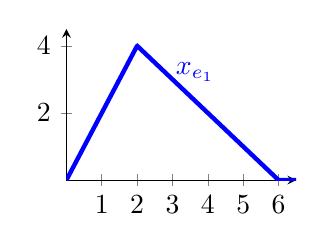
\begin{tikzpicture}[scale=1,solid,black,
	declare function={
		vol(\x)= (\x <= 2)*2*\x + and(\x > 2, \x <= 6)*(6-\x);			
	}]
	
	
	\begin{axis}[xmin=0,xmax=6.5,ymax=4.5, ymin=0, samples=500,width=4.5cm,height=3.5cm,
		axis x line*=bottom, axis y line*=left, axis lines=middle, xtick={1,2,3,4,5,6}]
		\addplot[blue, ultra thick,domain=0:7] {vol(x)} node[right,pos=.5]{$x_{e_1}$};
	\end{axis}
	
\end{tikzpicture}
\hspace{2cm}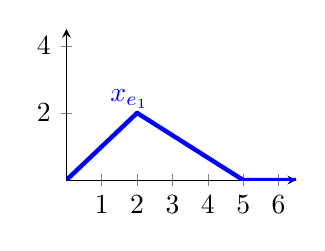
\begin{tikzpicture}[scale=1,solid,black,
	declare function={
		vol(\x)= (\x <= 2)*1*\x + and(\x > 2, \x <= 5)*(10/3-2/3*\x);			
	}]
	
	
	\begin{axis}[xmin=0,xmax=6.5,ymax=4.5, ymin=0, samples=500,width=4.5cm,height=3.5cm,
		axis x line*=bottom, axis y line*=left, axis lines=middle, xtick={1,2,3,4,5,6}]
		\addplot[blue, ultra thick,domain=0:7] {vol(x)} node[above,pos=.3]{$x_{e_1}$};
	\end{axis}
	
\end{tikzpicture}

		\caption{The flow volume $x_{e_1}(h,t)$ on edge $e_1$ given a constant inflow rate of $2$ (left) or $1$ (right) during the interval $[0,2]$. See \cite{CareyMcCartney} for more details on computing the flow dynamics with linear edge delays.}\label{fig:FlowVolumeGraph}
	\end{figure}
	
	Note, that a similar effect can be observed when using the Vickrey queuing model for the edge dynamics instead. Then, setting $\nu_e=1$ for all edges in the network gives us again an instance where sending all flow at a rate of $2$ into one of the two paths is feasible, while any convex combination of these two inflows violates the capacity constraint on edge~$e_3$.
\end{example}


Now, in order to adjust this example for the model used by Zhong et al. we make the following changes: We add an additional edge~$e_0$ with time-varying capacity constraint at the beginning forcing flow to arrive at node $v$ at a rate of $2$ even when departure time choice is enabled. Next, we replace the infinite service rate on edge $e_3$ by a large but finite service rate of $\frac{4}{\varepsilon}$ and slightly increase the capacity constraint on edge $e_3$ to $2+\varepsilon$. Finally, instead of a fixed inflow rate we now have a fixed flow volume $Q=4$. The resulting network is depicted in \Cref{fig:CounterExample}. 

\begin{figure}[h]
	\centering
	\input{tikz/CounterExample2.tex}
	%\includegraphics[width=.8\textwidth]{Images/CounterExample2.pdf}
	\caption{A counter example to \cite[Proposition 3.2]{zhong11}.}\label{fig:CounterExample}
\end{figure}

We first show that the capacity constraint on edge $e_0$ does indeed reduce the case with departure time to the case of fixed inflow rates:

\begin{claim}\label{claim:FlowOverEdge0}
	Let $h \in S$ be any feasible flow in the network depicted in~\Cref{fig:CounterExample} and $(f^+,f^-)$ its corresponding edge flow. Then, this flow enters edge $e_0$ at a rate of $4$ during the interval $[0,1]$ and leaves it at a rate of $2$ during the interval $[1,3]$ i.e. we have
		\[f^+_{e_0} \equiv 4\cdot\CharF[{[0,1]}] \text{ and } f^-_{e_0} \equiv 2\cdot\CharF[{[1,3]}] \text{ almost everywhere.}\]
\end{claim}

\begin{proofClaim}
	We first show that in a feasible flow all flow has entered edge $e_0$ by time $t=1$. So, let $t \coloneqq \min\set{\theta | \int_0^\theta f^+_{e_0}(\vartheta)\diff\vartheta = 4}$ be the time the last particle enters edge~$e_0$. We observe that due to the capacity constraint on edge $e_0$ all flow must have left edge $e_0$ by time $\theta = 3$. Thus, we must have 
	\[3 \geq t + D_{e_0}(h,t) = t + 1 + \frac{1}{4}\flowVolume[e_0](h,t)\]
	and, therefore, 
	\begin{align}\label{eq:CounterExampleA}
		\flowVolume[e_0](h,t) \leq 8-4t
	\end{align}
	as well as $t \leq 3-1=2$. Furthermore, since the total flow volume of $4$ must traverse edge $e_0$, at time $t$ we must have
	\begin{align}\label{eq:CounterExampleB}
		\int_0^t f^-_{e_0}(\vartheta)\diff\vartheta + \flowVolume[e_0](h,t) = 4.
	\end{align}
	Now, let $t'$ be the time at which particles have to enter edge $e_0$ in order to leave it at time $t$, i.e. $t'$ satisfies 
	\begin{align}\label{eq:CounterExampleE}
		t = t' + D_{e_0}(h,t') = t' + 1 + \frac{1}{4}\flowVolume[e_0](h,t').
	\end{align}		
	Since the edge travel time along edge $e_0$ is always at least $1$ we must have $t' \leq t-1 \leq 2-1 = 1$ and no particle has left edge $e_0$ by time $t'$. Thus, we have 
	\begin{align*}
		\flowVolume[e_0](h,t') = \int_0^{t'} f^+_{e_0}(\vartheta)\diff\vartheta \overset{\text{\eqref{eq:FlowConservationOnEdges}}}{=} \int_0^{t'+D_{e_0}(h,t')}f^-_{e_0}(\vartheta)\diff\vartheta = \int_0^t f^-_{e_0}(\vartheta)\diff\vartheta.
	\end{align*}
	Together with \eqref{eq:CounterExampleB} this gives us
	\begin{align}\label{eq:CounterExampleD}
		\flowVolume[e_0](h,t') = 4 - \flowVolume[e_0](h,t).
	\end{align}
	From this, we can now deduce
	\begin{align*}
		4t' = c_{e_0}(t') \geq \flowVolume[e_0](h,t') \overset{\text{\eqref{eq:CounterExampleD}}}{=} 4 - \flowVolume[e_0](h,t) 
		\overset{\text{\eqref{eq:CounterExampleA}}}{\geq} 4 - 8 + 4t = 4t-4
	\end{align*}
	and, thus,
	\begin{align*}
		4 \geq 4t - 4t' \overset{\text{\eqref{eq:CounterExampleE}}}{=} 4t' + 4 + \flowVolume[e_0](h,t') - 4t' = 4 + \flowVolume[e_0](h,t'),
	\end{align*}
	which gives us $\flowVolume[e_0](h,t') = 0$. Plugging this back into \eqref{eq:CounterExampleD} gives us $\flowVolume[e_0](h,t) = 4$ and, finally, feasibility of $h$ together with the the capacity constraint on edge $e_0$ then implies $t=1$ and, therefore,
		\begin{align}\label{eq:AllFlowEnteredByTime1}
			\int_0^\theta f^+_{e_0}(\vartheta)\diff\vartheta = 4 \text{ for all } \theta \geq 1.
		\end{align}
	
	Now, take any time $\theta \in [0,1]$ and let $\bar\theta \coloneqq \theta+D_{e_0}(h,\theta)$ be the time particles entering edge $e_0$ at time $\theta$ arrive at node $v$. Since $\bar\theta \in [1,3]$, the feasibility of $h$ implies
		\begin{align*}
			4-2\theta-\frac{\flowVolume[e_0](h,\theta)}{2} &= 6-2\left(\theta+1+\frac{\flowVolume[e_0](h,\theta)}{4}\right) = 6-2\bar\theta = c_{e_0}(\bar\theta) \\
				&\geq \flowVolume[e_0](h,\bar\theta) = \int_0^{\bar\theta}f^+_{e_0}(\vartheta)\diff\vartheta - \int_0^{\bar\theta}f^-_{e_0}(\vartheta)\diff\vartheta \overset{\text{\eqref{eq:AllFlowEnteredByTime1}}}{=} 4 - \int_0^{\bar\theta}f^-_{e_0}(\vartheta)\diff\vartheta \\
				&\overset{\text{\eqref{eq:FlowConservationOnEdges}}}{=} 4-\int_0^\theta f^+_{e_0}(\vartheta)\diff\vartheta = 4 - \flowVolume[e_0](h,\theta).
		\end{align*}
	which implies $\flowVolume[e_0](h,\theta) \geq 4\theta$.
	At the same time, feasibility of $h$ implies $\flowVolume[e_0](h,\theta) \leq 4\theta$ and, thus, we have $\flowVolume[e_0](h,\theta)=4\theta$ for all $\theta \in [0,1]$. Since no flow leaves edge $e_0$ before time $\theta=1$, this implies $\int_0^\theta f^+_{e_0}(\vartheta)\diff\vartheta = 4\theta$ and, therefore, $f^+_{e_0}(\vartheta) = 4$ for almost all $\vartheta \in [0,1]$. A direct computation then shows $f^-_{e_0}(\vartheta) = 2$ for almost all $\vartheta \in [1,3]$ as well.
\end{proofClaim}

Next, we define three path inflows: Flow $h^1$ sends flow into the upper path $e_0,e_1,e_3$ at a rate of $4$ during the interval $[0,1]$. Flow $h^2$ sends flow into the lower path $e_0,e_2,e_3$ at a rate of $4$ during the same interval. And, finally, $h^3$ splits the flow equally between the two paths, i.e. sends flow at a rate of $2$ into each of the two paths. We now claim that $h^1$ and $h^2$ are feasible while $h^3$ is not.

\begin{claim}
	In the network from \Cref{fig:CounterExample} the path inflows $h^1$ and $h^2$ are feasible. The path inflow $h^3$ is infeasible for $\varepsilon < \frac{2}{3}$.
\end{claim}

\begin{proofClaim}
	Both inflows $h^1$ and $h^2$ result in flow arriving at a rate of $1$ at node $w$ (without violating the capacity constraint on edge $e_0$ on the way). Since the total flow volume in the network is bounded by $4$, the travel time on edge $e_3$ is never larger than $2+\frac{4}{\frac{\varepsilon}{4}} = 2 + \varepsilon$. Thus, flow entering this edge at a rate of $1$ will never violate its capacity constraint. Therefore, both $h^1$ and $h^2$ are feasible.
	
	The equal split between the two paths in $h^3$ results in flow entering edge $e_1$ and $e_2$ at a rate of $1$ each during $[1,3]$. This flow exits these edges at a rate of $\frac{2}{3}$ during the interval $[3,6]$. Thus, the flow enters edge $e_3$ at a combined rate of $\frac{4}{3}$ during this interval. At particular at time $\theta=3+\frac{3}{4}\cdot(2+\varepsilon)$ a flow volume of $2+\varepsilon$ has entered edge $e_3$. If $\varepsilon < \frac{2}{3}$, this happens before time $\theta=5$ and, in particular, before any flow has left edge $e_3$. Thus, the total flow volume on edge $e_3$ is $2+\varepsilon$ at this time, leading to a violation of the capacity constraint immediately after.
\end{proofClaim}

Since $h^3$ is a convex combination of $h^1$ and $h^2$, this claim already shows the non-convexity of the set $S$ of feasible flows. To show that the variational inequality~\eqref{eq:ZhongVI} has no solution, we need the following additional property of all feasible flows in the given instance.

\begin{claim}
	Let $h \in S$ be any feasible path inflow for the instance in \Cref{fig:CounterExample}. Then, one of the two paths has a total inflow volume of at most $4\varepsilon$.
\end{claim}

\begin{proofClaim}
	Define $t_1$ as the last time a particle can enter edge $e_1$ under the flow induced by $h$ and still arrive by time $5$ at the node $w$ and define $t_2$ analogous for edge $e_2$. That is, we choose $t_1$ and $t_2$ such that we have
		\[t_1 + D_{e_1}(h,t_1) = 5 \quad\text{ and }\quad t_2 + D_{e_2}(h,t_2) = 5\]
	or, equivalently
	\begin{align}\label{eq:0}
		t_1 + \frac{x_{e_1}(h,t_1)}{2} = 3 \quad\text{ and }\quad t_2 + \frac{x_{e_2}(h,t_2)}{2} = 3.
	\end{align}
	Without loss of generality we assume that $t_1 \leq t_2$. Since $t_1,t_2 \leq 3 = \tau_{e_0}+\tau_{e_1} = \tau_{e_0}+\tau_{e_2}$, no flow has left edges $e_1$ and $e_2$ by time $t_2$ and, thus
	\[2(t_1-1) \overset{\text{\Cref{claim:FlowOverEdge0}}}{=} \int_0^{t_1}f^-_{e_0}(\theta)\diff \theta \leq x_{e_1}(h,t_1) + x_{e_2}(h,t_2).\]
	At the same time we also have
	\begin{align}\label{eq:4}
		x_{e_1}(h,t_1) + x_{e_2}(h,t_2) \leq x_{e_3}(h,5) \leq c_{e_2}(5) = 2+\varepsilon
	\end{align}
	since all this flow has entered edge $e_3$ by time $5$ but no flow has left it. Together, this implies $2(t_1-1) \leq 2 + \varepsilon$ and, therefore,
	\begin{align}\label{eq:1}
		t_1 \leq 2 + \frac{\varepsilon}{2}.
	\end{align}
	Since flow arrives at node $v$ at a rate of $2$ during $[1,3]$ (cf. \Cref{claim:FlowOverEdge0}), we also have
	\[x_{e_1}(h,t_1) \leq 2(t_1-1)\]
	while \eqref{eq:0} implies
	\begin{align}\label{eq:3}
		x_{e_1}(h,t_1) = 6 - 2t_1.
	\end{align}
	Together, this gives us $t_1 \geq 2$ which, combined with \eqref{eq:1}, results in $t_1 \in [2,2+\frac{\varepsilon}{2}]$. Using~\eqref{eq:3} we then get $x_{e_1}(h,t_1) \in [2-\varepsilon,2]$ and, with \eqref{eq:4},
	\[x_{e_2}(h,t_2) \leq 2 + \varepsilon - x_{e_1}(h,t_1) \leq 2 + \varepsilon - (2 - \varepsilon) = 2\varepsilon.\]
	Plugging this back into \eqref{eq:0} and solving for $t_2$ gives
	\[t_2 = 3 - \frac{x_{e_2}(h,t_2)}{2} \geq 3- \frac{2\varepsilon}{2} = 3-\varepsilon.\]
	Then, using again the fact that flow arrives at node $v$ at a rate of $2$ after time $\theta=1$, gives us
		\[x_{e_2}(h,3) \leq x_{e_2}(h,t_2) + 2\cdot(3-t_2) \leq 2\varepsilon + 2\varepsilon = 4\varepsilon.\]
	Since no flow leaves edge $e_2$ before time $3$ and no flow enters after time $3$, this proves our claim.
\end{proofClaim}

Now, let $h \in S$ be any feasible flow and $e_2$ the edge with a total inflow of at most $4\varepsilon$. We want to show that $\scalar{\Psi(h)}{h^2-h}<0$. Since the free flow travel times on both paths are equal, we only have to consider the additional flow dependent delays here (where the delays induced by flow $h$ in both cases). Furthermore, as both $h$ and $h^2$ are feasible flows, they are the same on edge $e_0$ (by \Cref{claim:FlowOverEdge0}). Thus, the delays experience on edge $e_0$ cancel out.
For flow $h^2$ edge $e_2$ contributes an additional delay of at most $\frac{4\varepsilon}{2}$ per particle and edge $e_3$ an additional delay of at most $\varepsilon$, leading to a total additional delay of at most $4\cdot(2\varepsilon+\varepsilon)=12\varepsilon$.
For flow $h$, on the other hand, a flow volume of at least $4-4\varepsilon$ traverses edge $e_1$ and is delayed there by all other particles using this edge (note, that by \Cref{claim:FlowOverEdge0} all particles enter edge $e_1$ during the interval $[1,3]$ and this edge has a travel time of at least $2$). Thus, the total additional delay here is at least
	\[\int_0^{4-4\varepsilon}\frac{x}{2}\diff x = 4-8\varepsilon+4\varepsilon^2.\]
This implies
	\[\scalar{\Psi(h)}{h^2-h} = \scalar{\Psi(h)}{h^2} - \scalar{\Psi(h)}{h} \leq 12\varepsilon - (4-8\varepsilon) = 20\varepsilon - 4\]
which is strictly smaller than $0$ for $\varepsilon<\frac{1}{5}$. Thus, for such $\varepsilon$ no feasible flow $h$ can be a solution to the variational inequality~\eqref{eq:ZhongVI}. 

Note, that whether or not the instances in \Cref{fig:CounterExampleConvexity,fig:CounterExample} \emph{should} have an equilibrium ought to depend on the behavioural model, i.e., which alternative strategies are available to individual particles under a given flow. However, a variational inequality of the form of~\eqref{eq:ZhongVI} cannot capture such subtleties as it essentially presents \emph{every} feasible flow as a potential alternative regardless of how different to the current flow it is. In particular, in the first example, the only existing alternative flow can be attained by a \emph{collective} deviation of all particles and, therefore, should not be relevant for an individual particle's choice. If, on the other hand, we only consider small ``$\varepsilon$-deviations'', the two feasible flows may very well be equilibria as no such small deviation leads to another feasible flow and, thus, individual particles have no potential alternative strategies.

\begin{framed}
	This discussion leads to the following key questions:
	\begin{itemize}
		\item What is a reasonable and useful definition of side-constrained equilibria for dynamic flows?
		\item Under which conditions can those equilibria be characterized by a variational inequality?
		\item Under which conditions is existence of such equilibria guaranteed?
	\end{itemize}
\end{framed}
We will try to provide answers to all three questions in the following three sections.
